\documentclass[11pt]{article}

\usepackage[a4paper,margin=1in]{geometry}
\usepackage{graphicx}
\usepackage{lscape}
\usepackage{tabularx}
\usepackage{booktabs}
\usepackage{url}
\usepackage{hyperref}
\usepackage{authblk}
\usepackage{color}
\usepackage{amsmath}
\usepackage{fancyvrb}
\usepackage{fontspec}
\setmainfont{TeX Gyre Pagella}
%\setmainfont{TeX Gyre Schola}
\setmonofont{Fira Code}

\title{%
\texttt{termal}: a fast and interactive terminal-based viewer for multiple sequence alignments
}

\author[1]{Thomas Junier}
\affil[1]{Swiss Institute of Bioinformatics, Vital-\textsc{it} Group, Bâtiment
Amphipôle, Quartier UNIL-Sorge, CH-1015 Lausanne, Switzerland\\
\texttt{thomas.junier@sib.swiss}}

\date{} % Actually _suppresses_ the date!

\begin{document}

\maketitle

\begin{abstract} \textbf{Summary:} We present \texttt{termal}, a fast,
  interactive terminal-based viewer for multiple sequence alignments (MSAs),
  designed for use on remote systems such as high-performance computing (HPC)
  clusters. Unlike traditional graphical viewers, \texttt{termal} runs entirely
  within a terminal and offers features such as scrolling, zooming,
  consensus/conservation visualization, and customizable color schemes. It is
  implemented in Rust, ensuring high performance and minimal dependencies.

	\textbf{Availability and implementation:} \texttt{termal} is written in Rust
	and freely available under the <INSERT> license at
	\url{gitlab.sib.swiss/tjunier/termal.git}

\end{abstract}

\section*{Introduction}

Visualising multiple sequence alignments (MSAs) is a common task in
computational biology. Many alignment viewers have a graphical user interface
(GUI) and are hence unsuitable for use on headless or remote systems such as
high-performance computing (HPC) clusters.  Command-line tools do exist, for
example Alan\cite{alan}, which stands out as a particularly elegant solution,
since it is built on standard Unix tools such as \texttt{awk} and \texttt{less}
--- indeed, it served as the initial inspiration for the present work. This
means, however, that Alan's interactivity is limited to that of a pager:
features such as zooming, reordering seqences, as well as computing and
displaying a consensus sequence are absent. While
\texttt{showalign}\cite{emboss} can compute a consensus, it does not support
coloring residues, and the user must explicitly call a pager in order to scroll
through the alignment. Other programs like \texttt{alen}\cite{alen} are
interactive, but not all have built-in residue colour schemes or the ability to
visually represent metrics such as similarity to the consensus, or to reorder
sequences according to such metrics. The capacity to fit a large alignment on
screen, typically by only displaying a subset of the sequences and columns, is
also rare (see also table~\ref{tbl:comparison}). In summary, text-based MSA
viewers collectively provide a substantial range of functions, but non viewer
implements all, or even most, of them. In this work we introduce
\texttt{termal}, which combines most of these features in a single application.

\section*{Interface}

Apart from the alignment sequences, which occupy the main pane, \texttt{termal}
also displays sequence labels and  ordinal numbers, a consensus sequence, and a
conservation bar plot; it also displays sequence metrics such as similarity to
the consensus, or (ungapped) length (figure~\ref{fig:screen}). The alignment can
be scrolled one sequence/column at a time using arrow keys or Vim-like
\texttt{h}, \texttt{j}, \texttt{k}, and \texttt{l}; similar keystrokes allow
jumping by screenfuls or to the edges of the alignment.

By default, residues of nucleotide aligmnents are coloured according to
Jalview's\cite{waterhouse2009jalview} nucleotide colour scheme, while protein
alignments use that of CLUSTALX\cite{larkin2007clustal}. An alternative color
scheme for protein is Lesk's\cite{lesk2019introduction}, and all alignments can
be rendered in monochrome. 

Alignments too wide to fit on the screen can be "zoomed out" by showing only the
first and last column, as well as a sample of equidistant columns in between.
The same can be done with sequences for aligments that are too tall. This
allows regions of high conservation to be spotted without scrolling. A variant
of the zoomed-out mode preserves the alignment's aspect ratio, at the cost of
some wasted space.

The sequences can be reordered according to the currently-displayed sequence
metric, in increasing or decreasing order. This allows e.g. to group the most
complete sequences together, or those that best match the consensus.

The width of the label pane can be adjusted to fit label length, and both the
side and bottom panes can be hidden to maximise the space allocated to the
alignment.

\texttt{termal} comes with a built-in help screen that lists all key bindings.

\begin{figure}[htbp]
\centering
	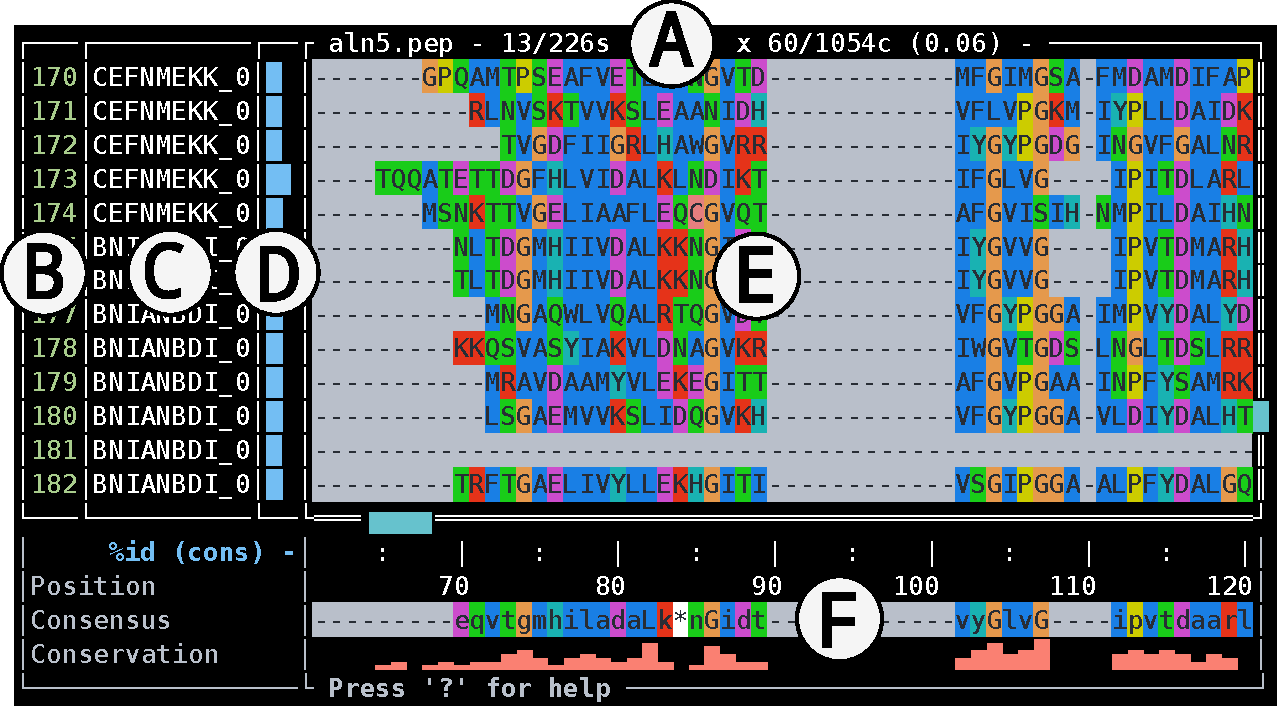
\includegraphics[width=\textwidth]{figure-1.pdf}
\caption{%
	A snapshot of \texttt{termal}'s interface showing a protein alignment. A:
	alignment filename and dimensions, B: sequence numbers pane, C: sequence
	labels pane, D: metric barplot pane (currently displaying sequence similarity
	with the consensus), E: alignment pane, F: bottom pane, displaying sequence
	position, consensus, and conservation barplot. \\
	In this example the sequences are in the original (file) order, and use the
	CLUSTALX color scheme. The view is zoomed in, that is, only a fracion of the
	alignment is displayed. }
	\label{fig:screen}
\end{figure}


\section*{Performance and Limitations}

\texttt{termal} has been tested on alignments exceeding 15,000 sequences and
1,500 columns (∼22 million alignment cells), with startup and initial rendering
completing in under one second on a machine with 12th-generation
Intel\textregistered{} Core\textsuperscript{TM} i5-1240P CPU and 16 GB of RAM
running Linux 6.14.2. In practice, interactive performance is limited more by
the speed of the terminal emulator than by \texttt{termal} itself.
GPU-accelerated terminals such as Alacritty\cite{alacritty}, Kitty\cite{kitty}
and Ghostty\cite{ghostty} offer smoother scrolling at large screen sizes than do
more traditional emulators.


\section*{Comparison with Existing Tools}

Table~\ref{tbl:comparison} presents a feature matrix for \texttt{termal} and a
selection of other TUI alignment viewers.

\begin{landscape}
\begin{table}[ht]
\centering
\small
\begin{tabularx}{\linewidth}{lXXXXX}
\toprule
\textbf{Feature} & \textbf{\texttt{termal}} & \textbf{\texttt{alen}} & \textbf{\texttt{alv}} & \textbf{\texttt{alan}} & \textbf{\texttt{showalign}} \\
\midrule
\textit{Basics} \\
Language & Rust & Rust & Python & Shell & C \\
Interactivity & Yes (full TUI) & Yes (TUI) & No (pager output) & No (pager output) & No (static output) \\
Handles large alignments & Yes (tested $>$15k$\times$1500) & Yes & Yes (slower) & Yes (but static) & Moderate \\
\midrule
\textit{Display features} \\
Scrolling / navigation & Yes & Yes & No & No & No \\
Zooming & Yes & No & No & No & No \\
Label pane toggle & Yes & No & No & No & No \\
Consensus display & Yes & Yes (reference toggle) & Yes (static) & No & Optional \\
Conservation display & Yes & No & No & No & No \\
Similarity histogram & Yes (vertical bars) & No & No & No & No \\
Color schemes & Multiple, configurable & Fixed & Fixed & Basic ANSI & Limited \\
Sequence numbering & Yes & No & No & No & Yes \\
Supported formats & FASTA & FASTA & FASTA, Clustal (via BioPython) & FASTA & FASTA, Clustal \\
\midrule
\textit{Sorting / filtering} \\
Sort by consensus similarity & Yes & No & No & No & No \\
Sort by sequence length & Yes & No & No & No & No \\
Manual row reordering & No & Yes & No & No & No \\
Regex search & No & Yes & No & No & No \\
\midrule
\textit{Integration / output} \\
Output style & TUI & TUI & STDOUT (to pager) & STDOUT (to pager) & Plain text output \\
HPC / CLI friendly & Yes (single binary) & Yes & Needs Python env & Yes & Yes (installed via EMBOSS) \\
	License & (TBD) & MIT & MIT & Various & GPL \\
\bottomrule
\end{tabularx}
\caption{Feature comparison of terminal-based MSA viewers.}
\label{tbl:comparison}
\end{table}
\end{landscape}

\section*{Availability}

\texttt{termal} is distributed under the <INSERT> license. It is available as a
single precompiled binary (for Linux, macOS, and Windows), with no external
dependencies or runtime environment required, from
\url{gitlab.sib.swiss/tjunier/termal.git}. Alternatively, users with Rust
installed can install it via \texttt{cargo install termal}.

\section*{Conclusion}

While this work is not intended as a comprehensive review of alignment viewers,
we surveyed several tools with comparable goals — namely, terminal-native
operation and varying degrees of interactivity — including \texttt{showalign},
\texttt{alan}, \texttt{alv}, and \texttt{alen}.  To our knowledge,
\texttt{termal} is the only tool to combine interactive navigation, zooming,
consensus and conservation visualization, and customizable layout options in a
single terminal interface.  Its minimal dependencies and fast startup make
\texttt{termal} suitable for both ad-hoc use and for integration into
semi-automated workflows requiring terminal-based alignment review. Accordingly,
\texttt{termal} fills a niche for fast, interactive MSA exploration directly in
the terminal, making it an ideal tool for remote bioinformatics workflows.

\section*{Acknowledgements}

The author wishes to thank Drs Guillaume Cailleau and Sébastien Moretti for
insightful comments on the program.

\bibliographystyle{plain} % or use plainnat, unsrt, etc.
\bibliography{termal}

\end{document}
